% vim: set fenc=utf-8 ft=latex encoding=utf-8
% -*- mode: latex; coding: UTF-8; -*-
%!TEX root = knowledge-curation.tex
\section{Methodology}
\label{cha:methodology}

The main goal of our study is to understand how knowledge is constructed and shared in both \SO and the \RH mailing list. To accomplish it, we decided to break
the study into the 
following research questions:
    \begin{enumerate}[label=\bfseries{RQ-\arabic*.},itemsep=3pt, topsep=2pt, leftmargin=3em, parsep=0pt]
        \item \rqa
        \item \rqb
        \item \rqc
     \end{enumerate}

To answer these questions we performed a qualitative case study of the knowledge that flows through both \RH and \SO. 
This research method is applicable when a concept or phenomenon requires more understanding, with little pre-existing research~\cite{Creswell2009}.

This study was composed
of two phases. In the first we did a random sampling of questions in both channels. Its purpose was to characterize the types of discussions that happen in both
channels. We sampled 400 questions in each channel; this sample guaranteed both saturation and a reliability of 95\% $\pm$ 5\%. The second phase was a survey of members of the R-community to obtain further additional insights and to verify our findings. 


\subsection{Phase 1: Understanding questions} 
\label{sec:studyDesign}

In this phase we mined both the archives of the R-users mailing list and \SO.

\subsubsection{Data collection and preparation}
\label{subsec:preparation}

We used the publicly available archives of both	the R-help mailing list and Stack Overflow. The R-Users mailing list dates started in 1997, while
the archives for Stack Overflow start in 2008 (when it was created).
To make both data sets comparable, we analysed both datasets from 2008 until 2013, a period of time that both channels were available.
For Stack Overflow, we obtained a data dump file available in its website. For the R-help mailing list data, we retrieved the archives available as MBOX files from the R website.

	We used two different software tools to prepare the data:
	\begin{enumerate*}[label=(\arabic*)]
	\item to process the Stack Overflow data, we used a modified version of Sam Saffron's application, So-Slow\footnote{\url{https://github.com/SamSaffron/So-Slow}}; and,
	\item to process the R-help mailing list archives, we wrote a our own mail mining application\footnote{Our tool is available at
            \url{https://github.com/cagomezt/GTMail}}, To ensure accurate results when processing the R-help mailing list, we followed the series of recommendations proposed by Bettenburg \textit{et al}.~\cite{Bettenburg2009}.
	\end{enumerate*}


%To make the data comparable againt the Stack Overflow dat set, we transformed the email addresses to MD5 hashes, and changed the time zone of the mailing list messages (UTC+2) to the time zone used by Stack Overflow (UTC).
    
Stack Exchange releases a new data dump from all their websites every three months\footnote{\url{http://stackexchange.com/sites}}.
However, the last dump file that containing email addresses as MD5 hashes was released in September 2013.
Since then, Stack Overflow does not provide the email addresses.
Because of this, we used the data dump file from September 2014, but updated the table \texttt{users} with the hashes in the dump file from September 2013, for whose \texttt{ID}s were identical in both data sets.
If a user from the 2013 data file did not exist in the 2014 data, we did not count it.
From \SO we retrieved all R-related data by selecting only messages with the R tag (\texttt{r}) and its synonyms\footnote{\url{http://stackoverflow.com/tags/r/synonyms}} (\texttt{rstats} and \texttt{r-language}).

	Table~\ref{table:data} depicts a summary of the data used for this study.
	The R-help has more questions, answers, and users than Stack Overflow, because there were approximately ten years of additional data.
	Only Stack Overflow's data contains ``comments'' information.

	\begin{table}[!htb]
	  \centering
      \caption{Raw data collected for each channel.}
      \begin{small}
        \begin{tabular}{lrr}
	        \toprule
	        Type          &  R-help & Stack Overflow \\
	        \midrule
	        Questions     & 101,931 &  67,393 \\
	        Answers       & 213,366 &  99,620 \\
	        Comments      &       - & 286,124 \\
	        Users         &  39,150 &  26,324 \\
	        \bottomrule
        \end{tabular}
      \end{small}
	  \label{table:data}
	\end{table}

To determine users who were common to both channels we compared the MD5 has of the participants of R-Users to the MD5s from \SO. Given the limitations of the
\SO data, we did not perform any unification fo email addresses, and therefore consider every email address to belong to a different individual. 
We found 1,421 different users (email addresses) on both media channels.

    % Although MD5 hashes are not \textit{collision resistant} and could possibly lead to false positives, it is unlikely that two different email addresses share a MD5 hash.



\subsubsection{Data analysis process}
\label{sec:dap}

    We performed an inductive approach~\cite{Runeson2012} to analyse the data from Stack Overflow and the R-help mailing list. 
    This is an iterative process, where across the study is necessary to switch between data selection and data analysis, or between data reporting and data collection.
    As advised to reduce bias~\cite{Runeson2012}, two researchers conducted the analysis, both computer scientists with a background in qualitative data analysis.
To answer RQ-1 and RQ-2, we selected 400 random threads of each channels.
To answer RQ-3, we studied questions that were posted with the same subject, sent to both channels, by same author. We found 79 threads and analyzed them all.
    
    \begin{figure*}[htbp]
    	\centering
    	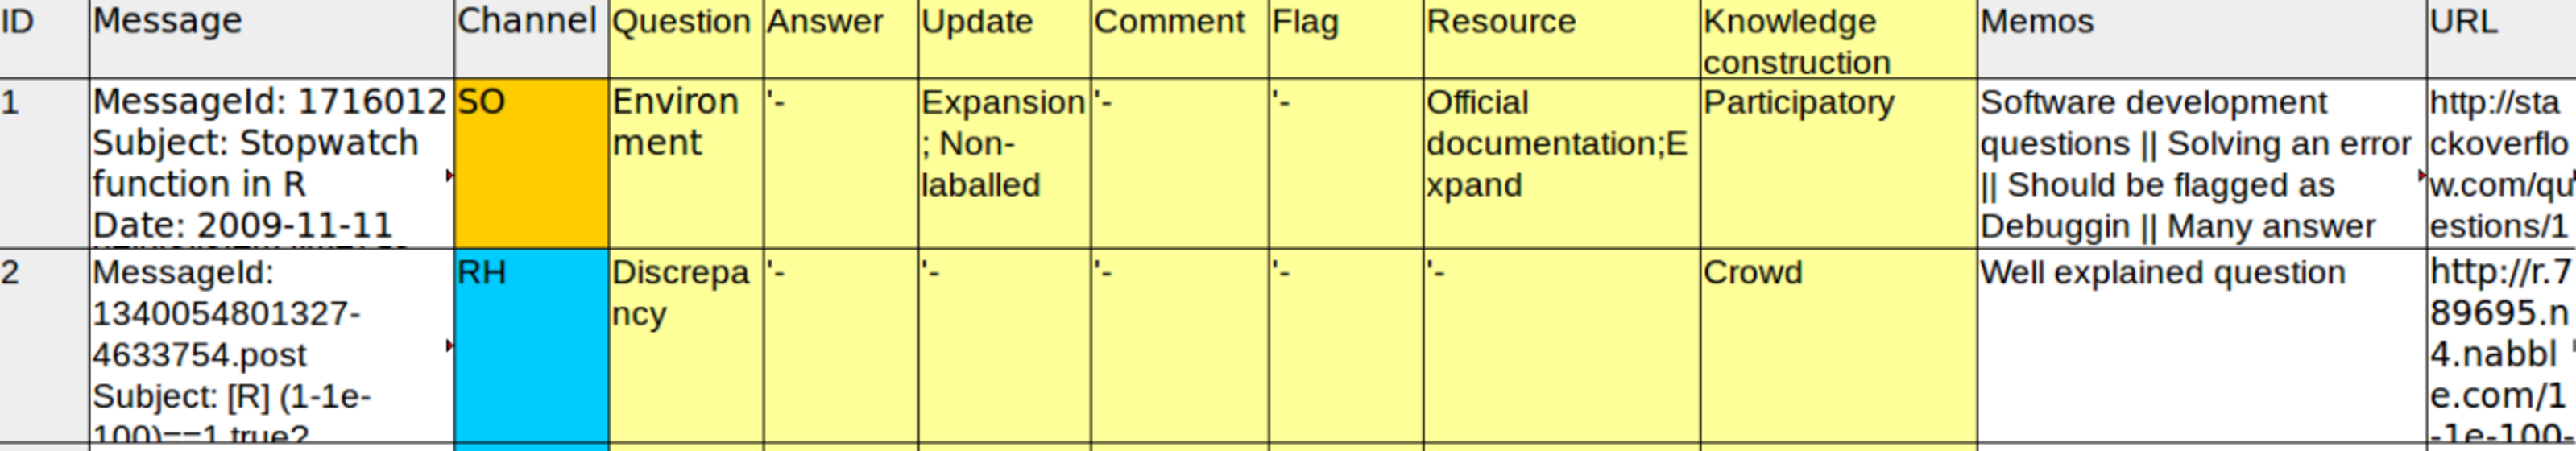
\includegraphics[width=.95\textwidth]{Figures/CodingExample}
    	\caption{Example of data coding. Each row is a thread message. Questions, comments, and answers are identified with the number on the first column. Columns in yellow contain the codification for each message type. The last two columns contain the memos and the URL.}
    	\label{fig:CodingExample}
\vspace{-3mm}
    \end{figure*}

    The techniques used to support the data analysis, which are explained as follow:

	\begin{description}[itemsep=2pt, topsep=0pt, leftmargin=1em, parsep=0pt]
		\item[Memoing] is the act of taking notes (coding) on what the researcher is learning from the data during the analysis~\cite{Groenewald2008}.
        We wrote reflective memos in a spreadsheet next to the applicable codes (see figure \ref{fig:CodingExample}).
        These memos were used to create the codes, and hypotheses about the relationships between concepts.

		\item[Affinity diagrams] allows to organize ideas and data into groups, and to find the relationships between concepts~\cite{Scupin1997}.
		We used them to discuss new insights, and while defining categories and relationships between them.

		\item[Inter-rater agreement \textit{Cohen Kappa}] is a coefficient used to measure the agreement between two coders who classify items into mutually exclusive categories~\cite{Stemler2004}.
		Ladis and Koch suggest that values above 0.60 or 60\% to obtain substantial results~\cite{Landis1977}.
		In a previous study~\cite{Gomez2013}, we used the same coefficient to measure agreement between coders.
		Based on this experience, we set a value above 0.80 or 80\% as the minimum to obtain substantial results.
		We used this coefficient after each coding session as a way to trigger discussion.

		\item[Code book] is a book that contains the definitions of the codes that researchers look during the data analysis~\cite{MacQueen1998}.
		We coded in multiple sessions, which allowed us to refine the definitions.
		Each entry is associated with a title, a formal definition, an example, and space for notes from the researcher.
		The final version of the code book is detailed in section~\ref{cha:findings}.
	\end{description}

	The focus of the analysis is to \textit{understand the context of the media channels and the community}.
	The process consisted of:
	First, a recollection of the official information for both channels and the community to build a background of the community of practice and the channels studied.
	Second, a mapping between messages from Stack Overflow with messages on the R-help mailing list.
    This is to overcome how the data is structured in both channels.
    The mapping of messages between both channels was as follows:

	\begin{description}[itemsep=3pt, topsep=2pt, leftmargin=1em, parsep=0pt]
		\item[Question:] the message is the first on the thread, and it contains the main question.
		\item[Answer:] the message provides a solution to the main question of the thread.
	 	\item[Update:] the message claims for a modification to a question (or answer) made by the author of such a question (or answer).
		\item[Comment:] the message offers a clarification to a specific part of the question or answer.
		\item[Flag:] the message requests attention from the moderator (e.g., repeated questions, spam, or rude behaviour).
	\end{description}

%	The data set was capped at 400 threads for each channel when we deemed our observations as being saturated.

\subsection{Phase 2: The survey} 

    We conducted a survey\footnote{A copy of the survey is available at \url{http://goo.gl/mxmH5J}} with members of the R community with the purpose of obtaining additional insights on the findings.
    To test and refine the questions, format and tone, we performed two pilots.
    
    We announced our survey on Twitter, Reddit, the R-help mailing list, and Meta Stack Exchange to reach users of both channels, and minimize the selection bias.
    However, on Stack Exchange the was deemed out of topic and was deleted a few minutes later. We received 26 valid responses.

%%% Local Variables:
%%% mode: latex
%%% TeX-master: "knowledge-curation.tex"
%%% End:
